% Fig. 1 of the report: the study pipeline (same diagram as the poster).
% Build: pdflatex fig_pipeline.tex  ->  fig_pipeline.pdf (vector, upload to Overleaf)
\documentclass[border=2pt]{standalone}
\usepackage[scaled]{helvet}
\renewcommand\familydefault{\sfdefault}
\usepackage{tikz}
\usetikzlibrary{positioning, arrows.meta, calc}
\definecolor{SUBlue}{HTML}{002F5F}
\definecolor{SUSky}{HTML}{ACDEE6}
% Numbered circle
\newcommand{\step}[1]{\tikz[baseline=(n.base)]\node[circle, fill=SUBlue, text=white, inner sep=0pt, minimum size=1.2em,
  minimum height=1.2em, text width=, align=center, draw=none, font=\bfseries\small] (n) {#1};}
\begin{document}
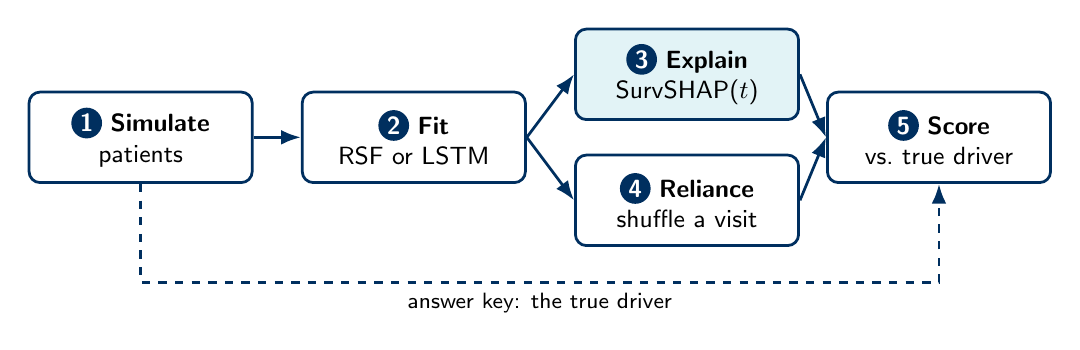
\begin{tikzpicture}[
    box/.style={draw=SUBlue, line width=1pt, rounded corners=4pt, fill=white, align=center,
                minimum height=1.15cm, text width=2.6cm, font=\small},
    key/.style={box, fill=SUSky!35},
    arrow/.style={-{Latex[length=2.5mm]}, line width=1pt, draw=SUBlue},
    lbl/.style={font=\footnotesize, align=center}]
  \node[box] (sim) {\step{1} \textbf{Simulate}\\patients};
  \node[box, right=0.6cm of sim] (fit) {\step{2} \textbf{Fit}\\RSF or LSTM};
  \node[key, right=0.6cm of fit, yshift=0.8cm] (run3) {\step{3} \textbf{Explain}\\SurvSHAP($t$)};
  \node[box, right=0.6cm of fit, yshift=-0.8cm] (run2) {\step{4} \textbf{Reliance}\\shuffle a visit};
  \node[box, right=3.8cm of fit] (score) {\step{5} \textbf{Score}\\vs.\ true driver};
  \draw[arrow] (sim) -- (fit);
  \draw[arrow] (fit.east) -- (run3.west);
  \draw[arrow] (fit.east) -- (run2.west);
  \draw[arrow] (run3.east) -- (score.west);
  \draw[arrow] (run2.east) -- (score.west);
  % Dashed: the answer key bypasses the model
  \draw[arrow, dashed] (sim.south) |- node[pos=0.75, below, lbl] {answer key: the true driver}
        ($(score.south) + (0, -1.25)$) -- (score.south);
\end{tikzpicture}
\end{document}
